% !TEX root = ../main.tex
% !TEX spellcheck = en_GB

\chapter{Analysis}
\label{chap:analysis}
To fulfil the specified requirements in \nameref{chap:requirements} a module to locate the system, save the location and send the location must be present.
Additionally a controller is needed to facilitate communication between the modules.
This system interfaces with a server as shown in \cref{fig:BDD:unspecified}

\begin{figure}[H]
	\centering
	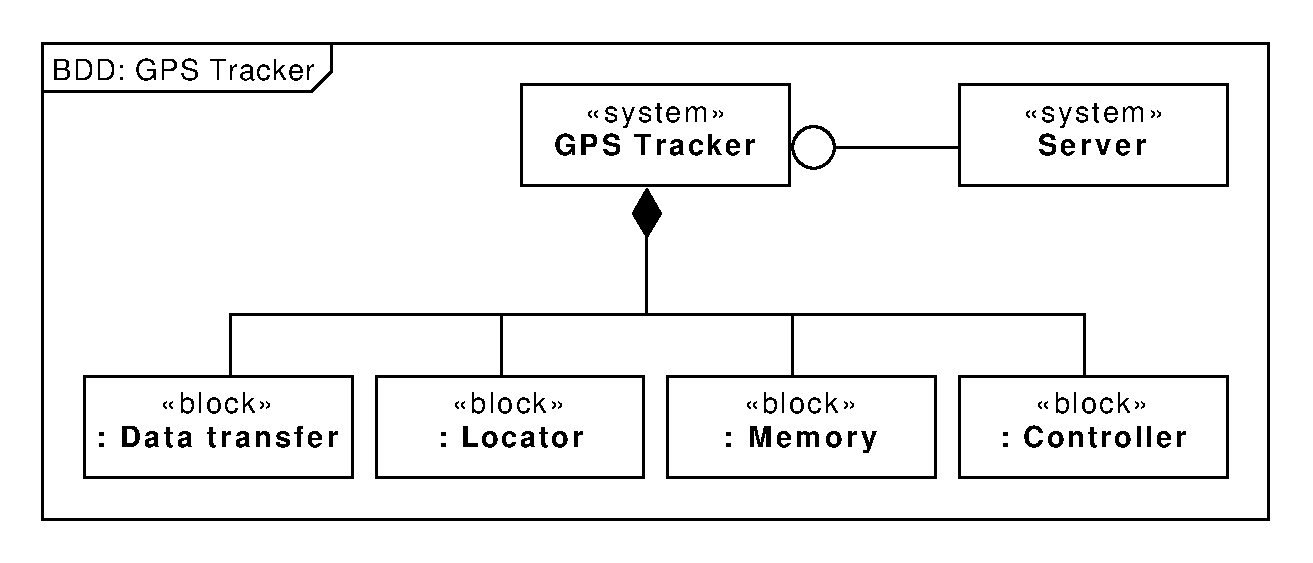
\includegraphics[width=0.7\linewidth]{gfx/Design/BDD_Unspecified.pdf}
	\caption{A high level BDD showing the parts of the \systemName and the interface with a server.}
	\label{fig:BDD:unspecified}
\end{figure}

\section{Controller}
The controller handles the interfacing between the other blocks.
It allows them to go into low power modes when not used, and wakes them up when necessary.
It should also, according to the requirements, be a low power device.
These specifications can be handled by a µC.
This fits very well with this project being part of a course on µC.

\section{Data Transfer}
The Data Transfer block is responsible for sending the data stored on the \systemName to a remote server for backup or analysis.
This can be done in a number of ways, most plausible are transmission over wifi, mobile networks or satellite.
\paragraph{Wifi} is very fast, but is also very limited in range and availability.
As this module is meant to be taken "on-the-move" the wifi technology does not offer the range required by the requirements section.
\paragraph{Mobile networks} be it GPRS, 2G, 3G or 4G, all offer long range communications available almost anywhere on the planet.
Modules are readily available, and the only requirement is the use of a SIM card, of which the acquisition and use is rather cheap.
As the data to be is merely GPS data, the amount of data sent could be low, and the speed of the chosen network should not be a focus.\fxnote{LoRaWAN?}
\paragraph{Satellite Internet access} is available anywhere on the planet.
It covers the globe using satellites, and the signal is only hindered by the weather.
The latency is high, \SI{638}{\milli\second} \cite{wiki:satellite}, but this should not be an issue in a system as this.
The drawbacks are that the equipment needed is rather large, and that the cost is \SI{300}{€} \cite{wiki:satellite}.
\paragraph{LoRaWAN} is a technology primarily developed to cater for the many IoT devices, which are developed at the time.
It offers low speeds but high ranges with few masts.
The issue with LoRaWAN is that it primarily covers urban areas, and coverage of out of town areas is minimal at the moment.

\section{Locator}
There are a few location services available, but one stands out.
\paragraph{GSM triangulation} uses available GSM masts, their location and their signal strengths to calculate and approximate location of the device.
This solution could possibly be paired with the Data Transfer module, allowing for fewer modules to be incorporated into the \systemName.
The issue with GSM triangulation is that the location accuracy drastically drops when GSM towers are not available or the reception settings are poor.
\paragraph{GNSS} is the go to solution for low power devices requiring knowledge of their location.
It is available world-wide and is free of charge, whether you choose the American GPS, Russian GLONASS or European GALILEO.
The accuracy is often less than \SI{10}{\metre}.

\section{Memory}
Storing memory is a vital function of the \systemName if the Data Transfer module is unable to establish a connection to the server, and to maximize power savings.
Storing data allows for only waking up the Locator module often, and save the data for transmission in larger packages.
\paragraph{EEPROM} grants access to a small volume of non-volatile data storage.
It might even be included on the chosen controller, allowing the Memory module to be internal.
An issue might be the storage volume, as the requirements specify at least \num{1440} data points.

\paragraph{USB Flash Drives} are readily available and the size of them is can be very small.
The available storage can be massive and is often in excess of \SI{1}{\giga\byte}. In order for a µM to interact with a USB drive, it will most likely need to use an external USB controller, which would be a secondary module needed.

\paragraph{SD cards} are very much like USB Flash Drives in that they can also store large amounts of data. SPI is a free to use interaction method with SD cards, which most µC can use.

\FloatBarrier
